\documentclass[standalone, version=1.0]{huangfusl-template}
\begin{document}
    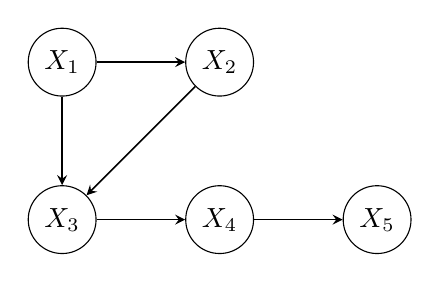
\begin{tikzpicture}
        \node[circle, draw] (X1) at (0, 0) {$X_1$};
        \node[circle, draw] (X2) at (2, 0) {$X_2$};
        \node[circle, draw] (X3) at (0, -2) {$X_3$};
        \node[circle, draw] (X4) at (2, -2) {$X_4$};
        \node[circle, draw] (X5) at (4, -2) {$X_5$};

        \draw[-stealth, semithick] (X1) -- (X2);
        \draw[-stealth, semithick] (X1) -- (X3);
        \draw[-stealth, semithick] (X2) -- (X3);
        \draw[-stealth, semithick] (X3) -- (X4);
        \draw[-stealth, semithick] (X4) -- (X5);
    \end{tikzpicture}
\end{document}